\setchapterpreamble[u]{\margintoc}
\chapter{Introduction} 
\labch{intro}

% Importance of multiphase interfacial flows 
\begin{marginfigure}
\centering
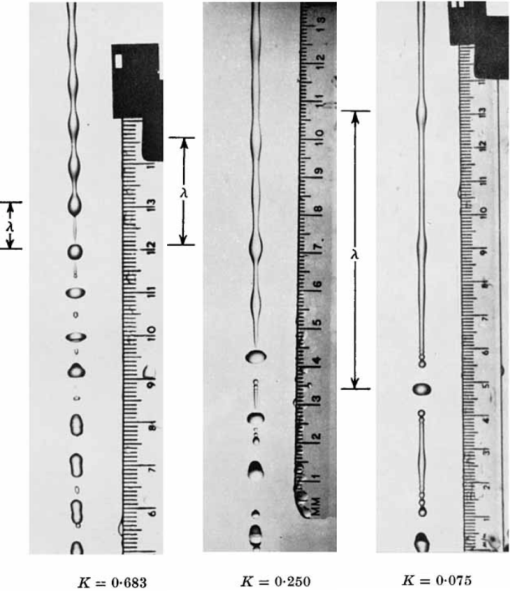
\includegraphics{plots/intro/jet.pdf}
\caption{Decay of a liquid jet into droplets due to the growth of capillary instabilities corresponding 
	to different excitation frequencies. Image reproduced from Rutland and Jameson \cite{rutland1971non}.
	} 
\label{jet}
\end{marginfigure}

The dynamics of liquid-gas interfacial flows play a critical role in several processes in nature, 
as well as in myriad industrial applications. 
The key elements of surface tension dominated flows such as droplets and bubbles constitute the  
fundamental mechanisms governing the exchange of heat and mass at the ocean-atmosphere interface \cite{seinfeld1998air,deike}, 
mixing/separation in context of metallurgical processes \cite{johansen1988fluid,metal},  
conventional modes of heat transfer \cite{deckwer1980mechanism,bubble}
and ever so importantly, the tranmission of pathogens \cite{lydia_1,lydia_2}. 
One of the most fascinating features of multiphase flows is the process of atomization, 
in which a liquid volume transitions into smaller fragments via a series of topological 
changes of varying complexity, ultimately resulting in the emergence of drops of various sizes
driven by the action of capillary forces at the interface separating the fluids.  
Such processes are ubiquitous in a diverse range of applications spanning from combustion related processes 
(\cite{lefebvre2017atomization,bayvel1993liquid}) to agricultural irrigation (\cite{lake1977effect,reichenberger2007mitigation}).    

% Decay of jets, shear induced atomization, expansion of sheets , hole expansion in sheets, secondary atomization of drops 

\begin{marginfigure}
\centering
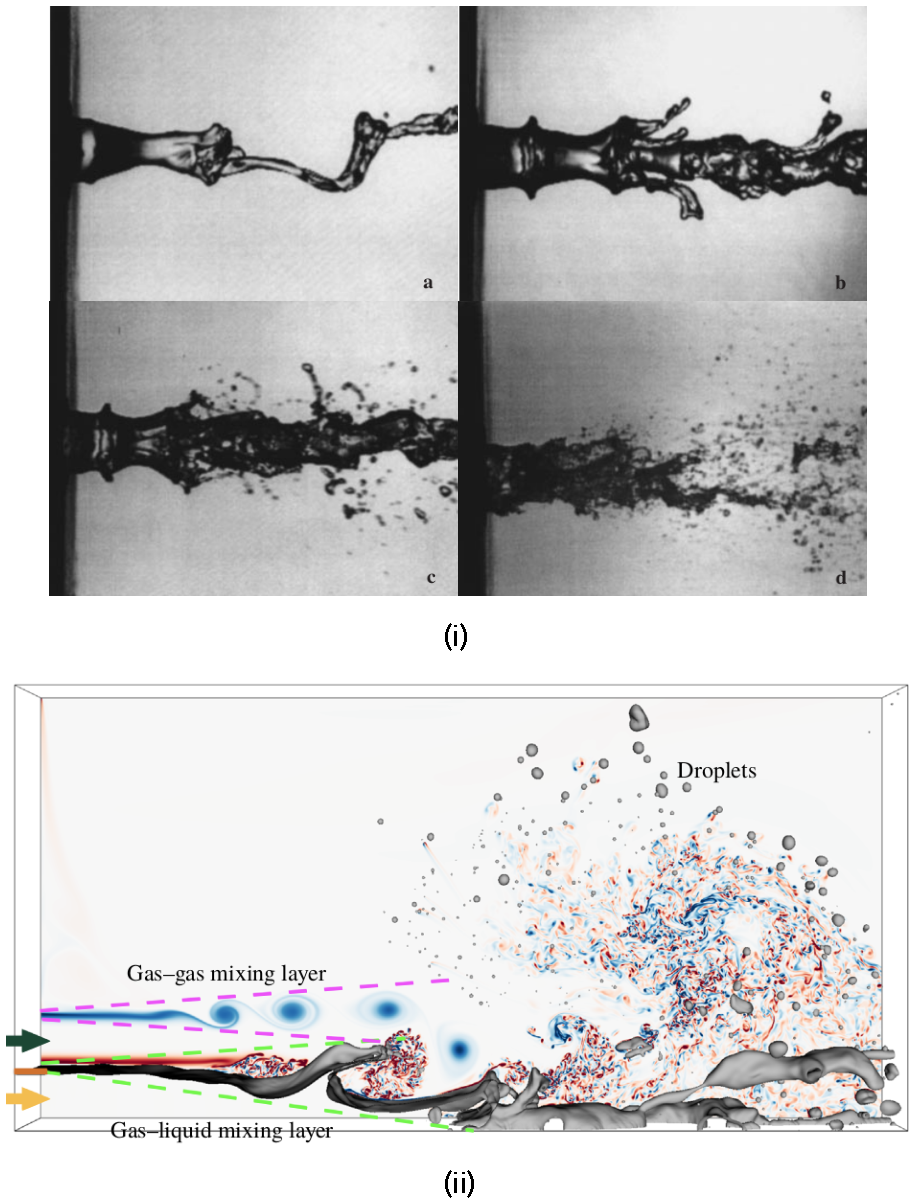
\includegraphics{plots/intro/shear.pdf}
	\caption{ Experimental and numerical investigations of liquid atomization 
	in which the primary stages of topological change are driven by shear instabilities. 
	(i) Liquid jet disintegration by a high speed coaxial gas flow, image reproduced from Lasheras and Hopfinger \cite{lasheras}.
	(ii) Atomization of a two-phase mixing layer between parallel liquid and gas streams, image 
	reproduced from Ling et al. \cite{ling}.
	}
\label{shear}
\end{marginfigure}

\Blindtext

\begin{marginfigure}
\centering
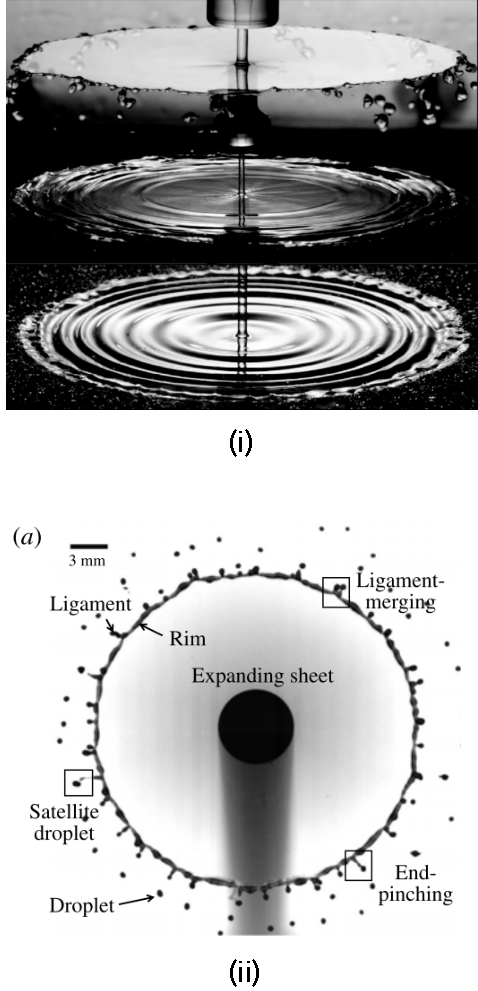
\includegraphics{plots/intro/spread.pdf}
	\caption{ Examples of steady and unsteady liquid fragmentation, demonstrating the disintegration of the  
	radially expanding liquid sheets driven by the capillary deceleration of the rims bounding the sheets. 
	(i) Steady fragmentation of radially expanding sheets driven by jet impact, image reproduced from Bremond et al. \cite{bremond}.
	(ii) Unsteady fragmentation of liquid sheets following drop impact, image reproduced from Wang and Bourouiba \cite{lydia_3}.  
	}
\label{spread}
\end{marginfigure}

\blindtext

\begin{marginfigure}
\centering
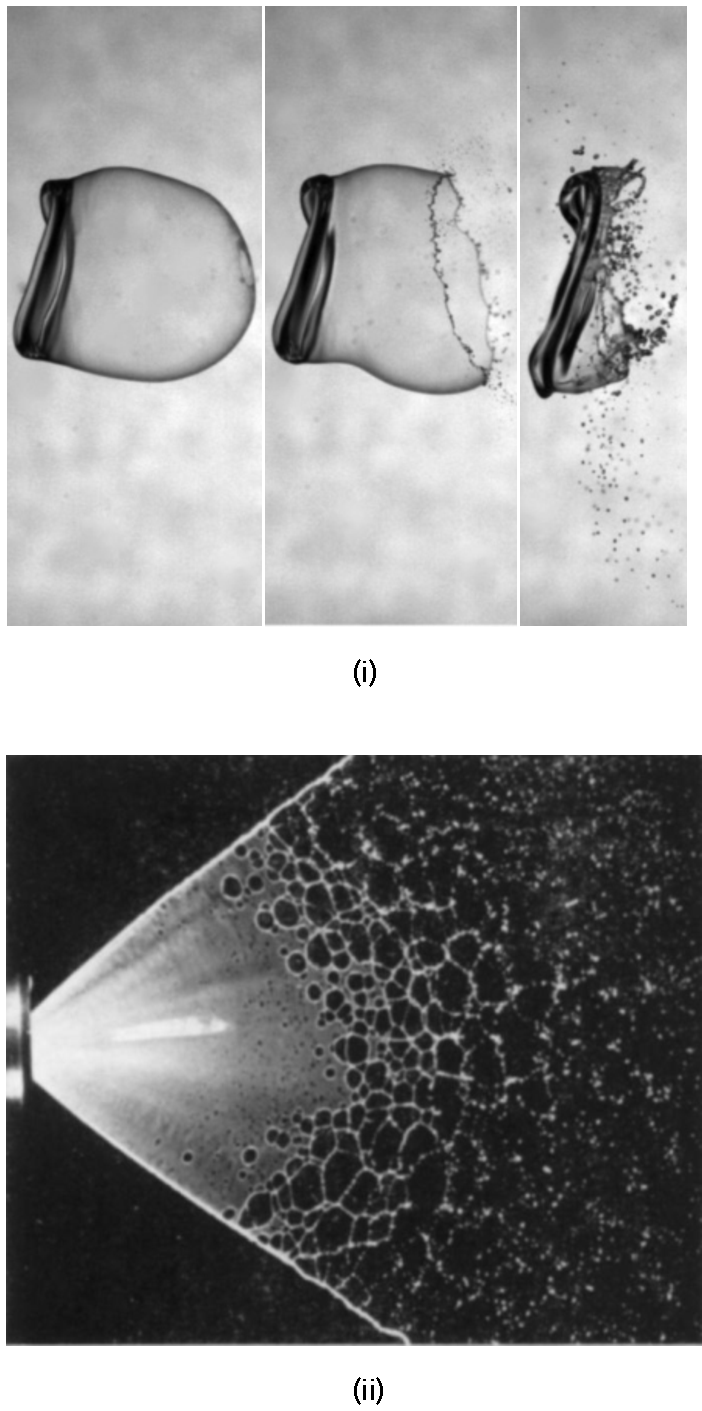
\includegraphics{plots/intro/holes.pdf}
\caption{ Liquid fragmentation triggered by the growth of perforations in thin liquid sheets. 
	(i) Secondary atomization (bag mode) of a drop in a crossflow, driven by the rapid capillary expansion of the hole. 
	Images reproduced from Opfer et al. \cite{hole_drop}.
	(ii) Effervescent atomization of expanding thin liquid sheets driven by the expansion of multiple perforations,
	image reproduced from Dombrowski and Fraser \cite{hole_sheet}.
	}
\label{holes}
\end{marginfigure}

\section*{Challenges in Numerical Modeling}

% Utility of numerical simulations, general info on interfacial tracking, Navier-Stokes 

% Artifical Atomization at low resolutions (raindrop crashes).

% Literature review of different attempts at momcons + summary tables

% Our Approach 


\section*{Polydispersity in Drop Sizes}

% Ligament mediated paradigm
% Breakup Regimes : Keller-Miksis inviscid, Paparouglou viscous, Eggers universal (inertio-visco) 

% Log-Normal, Gamma , Poisson distributions and underlying mechanisms

% Our approach


% Summary of parts and chapters in thesis
